\noindent
\begin{figure}[ht!]
  \centering
  \begin{subfigure}[t]{0.5\textwidth}
  	\centering
    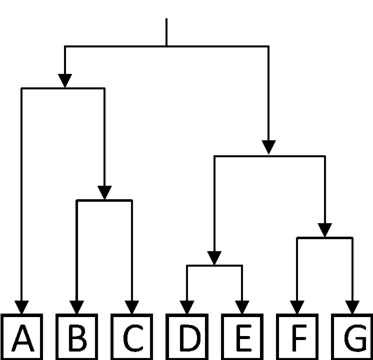
\includegraphics[width=0.40\textwidth]{hierarchical-clustering-example2}
    \caption{}
	%\caption{Hierarchical clustering example. The partial relation exists only between clusters.} 
	\label{fig:hierarchical-example} 
  \end{subfigure}%
  ~
  \begin{subfigure}[t]{0.5\textwidth}
  	\centering
    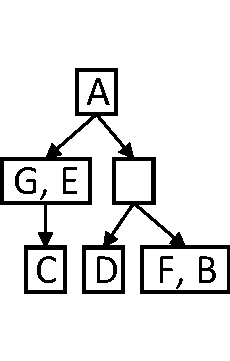
\includegraphics[width=0.40\textwidth, trim={0 1.15cm 0 1.15cm}, clip]{OCH-clustering-example}
    \caption{}
	%\caption{Object Cluster hierarchy example. The partial relation exists between both the clusters and the objects.}
	 \label{fig:och-example} 
  \end{subfigure}
  \caption{Dendrogram (a) and Object Cluster Hierarchy (b) examples. Letters represent objects and squares are groups. The arrows show the partial order relation. In the Dendrogram, the partial relation exists between both the clusters and the objects, whereas in the Object Cluster Hierarchy the partial relation exists between both the clusters and the objects.}
\end{figure}